% This text is abandoned but kept here for archiving.

\subsection{Pyramid amortized R-CNN}\label{sec:dense}

Another fast ROI featurization we consider is a variant of R-CNN that processes the whole image, at multiple scales, with the CNN up to the topmost non-fully-connected layer.
We call this multiscale CNN output a ``feature pyramid''.
As \autoref{fig:dense_rcnn} shows, ROIs are then cropped from the feature pyramid at the best matching scale, warped to a canonical size, and classified.
ROIs are highly overlapping, but their featurization is shared through the pyramid, amortizing its construction cost.
This doesn't work as well as the original R-CNN system, but is much faster, and can therefore be used as the fast feature for the dynamic region selection.

% \subsubsection{Design choices}

We explored a variety of choices while designing Pyramid R-CNN.
We tried using a single scale or a pyramid with 7 levels each separated by a scale factor of $2^{-1/2}$.
For warping, we experimented with canonical sizes of $s \times s$, for $s \in \{5,6,7\}$ and resampling with nearest neighbor or bilinear interpolation.
We also tried two variants of the feature pyramid: the raw feature pyramid or one where each level is max pooled with a $3 \times 3$ pooling window run at a stride of $1$ (to avoid subsampling).

\autoref{tab:prcnn} shows mAP performance on PASCAL VOC 2007 test for these various choices.
The best configuration, in terms of mAP, uses a 7 level pyramid, a warp size of $7 \times 7$ with bilinear interpolation, and max pooling.
The first level of our pyramid is computed from a $1713 \times 1713$ pixel image, which yields a $108 \times 108$ cell feature map.
The gold standard (non-pyramid) R-CNN performance using the same non-fine-tuned CNN is 44.2\% mAP.
Our best result with Pyramid R-CNN is slightly worse, at 41.9\%.

To map a ROI $R$ into the pyramid, we start by computing an ``optimal'' scale defined by $\alpha^* = 227/\min(h,w)$, where $h$ and $w$ are image height and width of $R$.
We then find the nearest level in the pyramid: $l^* = \textrm{argmin}_l |\log(\alpha_l) - \log(\alpha^*)|$, where $\alpha_l$ is the scale factor for pyramid level $l$.
This procedure approximates the scale that R-CNN would use, since it operates on $227$ pixel inputs.

\begin{table}[ht]
\centering
\caption{
    Pyramid R-CNN design choices, vs mAP performance.
    We additionally show two best and two worst performing classes.
}\label{tab:prcnn}
\small{
\begin{tabular}{@{}rccccl@{}}
\toprule
settings      & \mcell{warp 7x7\\nearest}  & \mcell{warp 7x7\\nearest}  & \mcell{warp 7x7\\bilinear}  & \mcell{max pooled 3x3\\warp 7x7\\bilinear} \\
scales        & 1                          & 7                           & 7                          & 7 \\
\midrule
aeroplane     & 31.7                       & 46.8                        & 44.5                       & 47.0 \\
bicycle       & 36.1                       & 50.1                        & 52.6                       & 57.9 \\
bird          & 12.3                       & 25.4                        & 26.7                       & 31.1 \\
boat          & 12.5                       & 20.4                        & 25.7                       & 27.5 \\
bottle        & 11.4                       & 12.9                        & 12.6                       & 19.8 \\
bus           & 17.1                       & 43.6                        & 45.4                       & 50.7 \\
car           & 39.8                       & 54.3                        & 56.7                       & 60.0 \\
cat           & 7.0                        & 39.0                        & 42.4                       & 48.2 \\
chair         & 6.7                        & 11.7                        & 11.8                       & 16.0 \\
cow           & 25.8                       & 41.9                        & 44.1                       & 50.1 \\
diningtable   & 10.2                       & 29.2                        & 33.0                       & 38.6 \\
dog           & 7.2                        & 35.3                        & 36.0                       & 41.6 \\
horse         & 17.3                       & 46.3                        & 51.2                       & 55.8 \\
motorbike     & 27.8                       & 49.4                        & 53.3                       & 56.6 \\
person        & 16.6                       & 28.8                        & 31.3                       & 36.4 \\
pottedplant   & 11.4                       & 17.1                        & 18.6                       & 20.9 \\
sheep         & 19.3                       & 34.4                        & 35.8                       & 40.2 \\
sofa          & 10.3                       & 22.8                        & 29.3                       & 35.8 \\
train         & 17.9                       & 38.1                        & 43.0                       & 44.9 \\
tvmonitor     & 36.3                       & 50.0                        & 54.0                       & 59.7 \\
\midrule
mAP           & 18.7                       & 34.9                        & 37.4                       & 41.9 \\
\bottomrule
\end{tabular}

}
\end{table}

\begin{figure}[h!]
\begin{center}
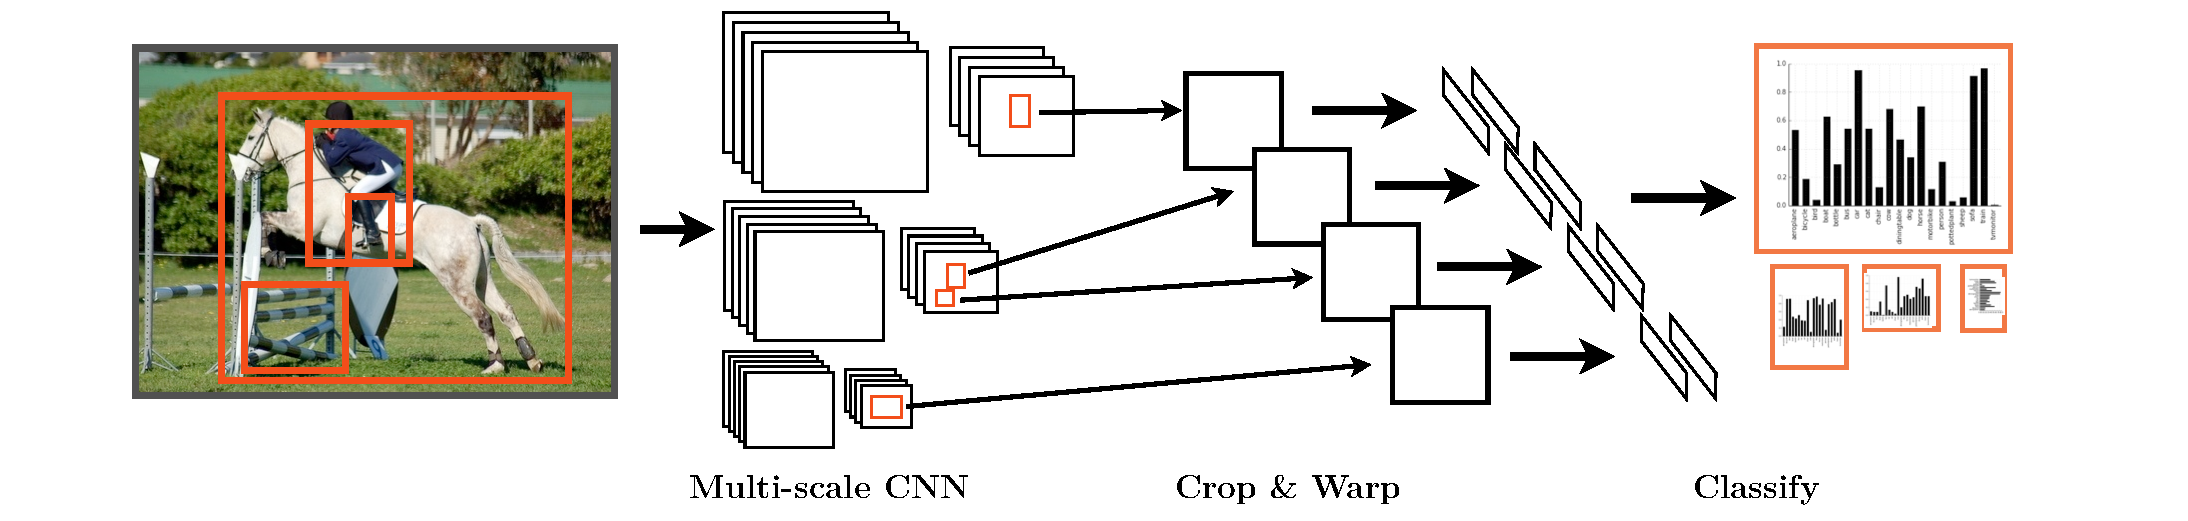
\includegraphics[width=0.98\columnwidth]{figures/dense_rcnn.pdf}
\caption{
Post R-CNN architecture: the whole image is fed through a CNN up to the highest pooling layer.
Regions are cropped from that layer at the best matching scale, resized, and classified.
}\label{fig:dense_rcnn}
\end{center}
\end{figure}
